% vim:encoding=utf8 ft=tex sts=2 sw=2 et:


\documentclass{classrep}
\usepackage[utf8]{inputenc}

\usepackage[pdftex]{color,graphicx}
\DeclareGraphicsExtensions{.pdf,.png,.jpg}

\usepackage{float}

\usepackage{color}

\usepackage{listings}

\usepackage{color}

\usepackage[hyphens]{url}

\usepackage{hyperref}

\usepackage[polish]{babel}

\usepackage{enumitem}


\usepackage{indentfirst}
\usepackage[center,small,bf]{caption}
\hypersetup{colorlinks=false,pdfborder={0 0 0}}

\renewcommand{\labelitemi}{$\bullet$}
\renewcommand{\labelitemii}{$\cdot$}
\renewcommand{\labelitemiii}{$\diamond$}
\renewcommand{\labelitemiv}{$\ast$}
\definecolor{dkgreen}{rgb}{0,0.6,0}
\definecolor{gray}{rgb}{0.5,0.5,0.5}
\definecolor{mauve}{rgb}{0.58,0,0.82}
\lstset{ %
  language=Matlab,                % the language of the code
  basicstyle=\footnotesize,           % the size of the fonts that are used for the code
  numbers=left,                   % where to put the line-numbers
  numberstyle=\tiny\color{gray},  % the style that is used for the line-numbers
  stepnumber=2,                   % the step between two line-numbers. If it's 1, each line 
                                  % will be numbered
  numbersep=5pt,                  % how far the line-numbers are from the code
  backgroundcolor=\color{white},      % choose the background color. You must add \usepackage{color}
  showspaces=false,               % show spaces adding particular underscores
  showstringspaces=false,         % underline spaces within strings
  showtabs=false,                 % show tabs within strings adding particular underscores
  frame=single,                   % adds a~frame around the code
  rulecolor=\color{black},        % if not set, the frame-color may be changed on line-breaks within not-black text (e.g. commens (green here))
  tabsize=2,                      % sets default tabsize to 2 spaces
  captionpos=b,                   % sets the caption-position to bottom
  breaklines=true,                % sets automatic line breaking
  breakatwhitespace=false,        % sets if automatic breaks should only happen at whitespace
  title=\lstname,                   % show the filename of files included with \lstinputlisting;
                                  % also try caption instead of title
  keywordstyle=\color{blue},          % keyword style
  commentstyle=\color{dkgreen},       % comment style
  stringstyle=\color{mauve},         % string literal style
  escapeinside={\%*}{*)},            % if you want to add a~comment within your co
}

\studycycle{Informatyka, studia dzienne, mgr II st.}
\coursesemester{I}

\coursename{Metody obliczeniowe optymalizacji}
\courseyear{2011/2012}

\courseteacher{mgr inż. Łukasz Chomątek}
\coursegroup{czwartek, 16:00}

\author{
  \studentinfo{Paweł Musiał}{178726} \and
  \studentinfo{Łukasz Michalski}{178724}
}

\title{Zadanie 3: Optymalizacja wielowymiarowa bez ograniczeń} % np \title{Zadanie 1: Optymalizacja jednowymiarowa}
\svnurl{https://serce.ics.p.lodz.pl/svn/labs/moo/lc_cz1600/lmpm}

\begin{document}
\maketitle

\section{Cel}
Zaimplementować jedną spośród następujących metod optymalizacji:
\begin{itemize}
\item pełzający sympleks
\item  metoda Fletchera-Reevesa
\item \textbf{metoda quasi-Newtona w wersji Davidon-Fletcher-Powell (DFP)}
\end{itemize}
Przedstawiany jako rozwiązanie program powinien prezentować kolejne kroki poszukiwania rozwiązania.

\section{Rozwiązanie zadania}
Metody ,,quasi-newtonowskie'' są metodami wyznaczania lokalnych ekstremów funkcji. Metoda ta oblicza postać przybliżoną macierzy Hessego, przy pomocy gradientu. Kolejne przybliżenia rozwiązania wyznaczamy w następujący sposób.

Informacja o wartości macierzy Hessego w punkcie daje nam dane o krzywiźnie funkcji. Jeśli macierz ta jest dodatnio określona w punkcie to oznacza, że jest to lokalne minimum, natomiast gdy jest ujemnie oznaczona oznacza to, że w danym punkcie znajduje się lokalne maksimum. W przypadku gdy macierz jest nieokreślona ma miejsce punkt przegięcia.

\begin{enumerate}
\item Inicjalizacja
	\begin{itemize}
		\item ustal dodatnio określoną macierz $S_0$
		\item punkt początkowy $x_0$
		\item licznik $k=0$
	\end{itemize}
\item Iteracja
	\begin{itemize}
		\item oblicz $g_k = \nabla f(x_k)$
		\item oblicz $d_k = -S_k g_k$
		\item wyznacz $\alpha _k$ metodą Wolfe
		\item przypisz $x _{k+1} = x_k + \alpha _k d _k$
		\item Aktualizacja przybliżenia macierzy Hessego
		 \begin{itemize}
		 	\item oblicz $p_k = \alpha _k d _k ; g _{k+1} = \nabla f(x_{k+1})$
		 	\item oblicz $q_k = g_{k+1}-g_k$
		 	\item oblicz $S_{k+1}= S_{k} + \frac{p_{k}p_{k}^{T}}{< p_{k} , q_{k} >} - \frac{S_{k} q_{k} q_{k} ^{T} S_k }{< q_{k} , S_{k} q_{k}  >}$
		
		\end{itemize}
		\item przypisz $k=k+1$
	\end{itemize}
\end{enumerate}

Gdzie warunkiem stopu algorytmu jest albo liczba iteracji, albo wielkość kroku.

Kryterium Wolfa, jest rozszerzeniem kryterium poprawy Armijo
\begin{equation}
f( x^{k} + \lambda ^{k} d^{k} ) \leq f(x^{k}) + c \lambda ^{k} \nabla f^{T} (x ^{k} ) d^{k}
\end{equation}
 o kryterium krzywizny:
\begin{itemize}
\item Słabe kryterium krzywizny\\
	\begin{equation}
	\nabla f^{T} (x^{k} + \lambda ^{k} d^{k} ) d^{k} \geq c \nabla f^{T} (x ^{k} ) d^{k}
	\end{equation}
	
\item Silne kryterium krzywizny\\
	\begin{equation}
	\| \nabla f^{T} (x^{k} + \lambda ^{k} d^{k} ) d^{k} \| \leq \| c \nabla f^{T} (x ^{k} ) d^{k} \|
	\end{equation}

\end{itemize}

Gdzie :
\begin{itemize}
 \item $x^k$ - kolejne przybliżenia rozwiązania
 \item $\lambda ^k$ - długość kroku
 \item $d ^k$ - kierunek zmiany
 \item $c$ - stałe używane w kryteriach
 \item $f(x)$ - wartość funkcji podstawowej w punkcie
 \item $\nabla f(x)$ - wartość gradientu w punkcie
\end{itemize}

Dobór długości kroku na podstawie kryterium Wolfe odbywa się przy pomocy algorytmu backtrakingu:
\begin{enumerate}
\item Sprawdź czy zachodzi kryterium dla zadanej długości kroku
\item Jeśli kryterium zachodzi, zwróć długość kroku $\lambda$
\item Jeśli kryterium nie zachodzi, oblicz $\lambda =\lambda \rho$, gdzie $\rho \in (0,1)$ , wróć do punktu 1
\end{enumerate}

\section{Opis programu}
Program jest implementacją wyżej opisanej metody. Wyjaśnienie znaczenia zmiennych :
\begin{itemize}
\item \textbf{f0} - funkcja podstawowa
\item \textbf{f1} - gradient funkcji
\item \textbf{d} - kierunek zmiany
\item \textbf{x} - kolejne przybliżenia
\item \textbf{a} - długość kroku
\item \textbf{c} - parametr kryterium
\item \textbf{Sk} - kolejne przybliżenia macierzy Hessego
\item \textbf{rho} - parametr backtrackingu
\end{itemize}
\subsection{Metoda Quasi-newtona DFP}

\begin{lstlisting}{metoda quasi-newtona DFP}
function x=dfp(x0,fn,a0,rho,c,kMax, eps)
f=inline(fn);
f0=@(x)f(x(1),x(2));
syms x y
t=[x;y];
w=fn;
gfn=matlabFunction(jacobian(w,t).');
f1=@(x)gfn(x(1),x(2));
sl='wolfe';
sl=@(x,d)backtk(sl,a0,x,d,c,f0,f1,rho);
x=x0;
k=0;

Sk = eye(length(x0), length(x0));
err = 1.0;
X=x(1);
Y=x(2);
fk=0;
while (k<kMax) && (eps < err)
    g = f1(x);
    d = -Sk*g;
    a=sl(x,d);
    fk = f0(x);
    x=x+a*d;
    fprintf('f(%.3f,%.3f)=%.3f\n',x(1),x(2),fk);
    fk_new = f0(x);
    p = a*d;
    q= f1(x) - g;
    Sk = Sk + (p*(p'))/(p'*q) - (Sk*q*(q')*Sk)/(q'*(Sk*q)); 
    k=k+1;
    err = max( abs(fk - fk_new),norm(p));
end
\end{lstlisting}

\subsection{Kryterium Wolfe}

\begin{lstlisting}{Slabe kryterium Wolfa}
if c(1)*f1(x)'*p<=f1(x+a*p)'*p &&
 f0(x+a*p)<=f0(x)+c(2)*a*f1(x)'*p
    test=1;
else 
    test=0;
end
\end{lstlisting}

\begin{lstlisting}{Silne kryterium Wolfa}
if abs(c(1)*f1(x)'*p)>=abs(f1(x+a*p)'*p) &&
 f0(x+a*p)<=f0(x)+c(2)*a*f1(x)'*p
    test=1;
else 
    test=0;
end
\end{lstlisting}

\subsection{Algorytm backtrackingu}

\begin{lstlisting}{Algorytm backtrackingu}
switch cond
    case 'wolfe'
        check=@(a) wolfe(a,x,p,c(1),f1) &&
        			 armijo(a,x,p,c(2),f0,f1);
    case 'wolfes'
        check=@(a) wolfes(a,x,p,c(1),f1) &&
        			 armijo(a,x,p,c(2),f0,f1);
end
a=a0;
while check(a)~=1 && abs(a) > 0.0000001
    a=rho*a;
end
\end{lstlisting}

\section{Wyniki}

Testowana funkcja : $x^2+y^2$\\
Dla Argumentów : $[2;1]$, $x^2+y^2$, $0.6$, $0.99$, $[0.6;0.4]$, $100$, $0.001$\\
Kolejne przybliżenia:
\begin{enumerate}
\item f(-0.400,-0.200)=5.000
\item f(-0.160,-0.080)=0.200
\item f(-0.064,-0.032)=0.032
\item f(-0.026,-0.013)=0.005
\item f(-0.010,-0.005)=0.001
\item f(-0.004,-0.002)=0.000
\item f(-0.002,-0.001)=0.000
\item f(-0.001,-0.000)=0.000
\item f(-0.000,-0.000)=0.000
\end{enumerate}

\begin{figure}[H]
\centering
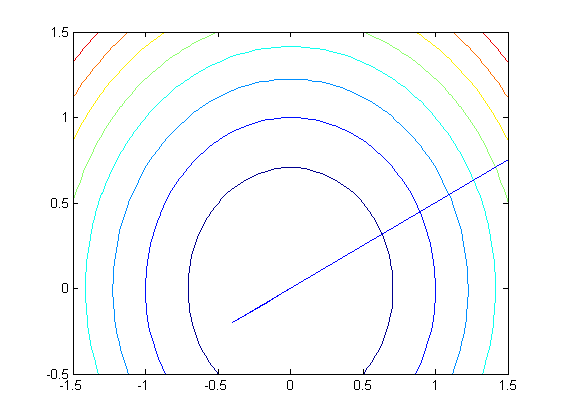
\includegraphics[width=12cm]{fcja1} 
\caption{Wykres kolejnych przybliżeń dla funkcji $x^2+y^2$.}
\label{fig:funkcja_1}
\end{figure}

Testowana funkcja : $x + 10*x - x^5 + y + 10*y^3 - y^5$\\
Dla Argumentów : $[1;2]$, $x + 10*x - x^5 + y + 10*y^3 - y^5$, $0.6$, $0.99$, $[0.6;0.4]$, $15$, $0.00001$\\
Kolejne przybliżenia:
\begin{enumerate}
\item f(0.272,-2.977)=60.000
\item f(-1.014,-2.301)=-30.053
\item f(-1.296,-2.313)=-69.709
\item f(-1.296,-2.313)=-70.454
\item f(-1.254,-2.415)=-70.454
\item f(-1.234,-2.444)=-71.809
\item f(-1.225,-2.452)=-71.942
\item f(-1.221,-2.454)=-71.955
\item f(-1.219,-2.456)=-71.958
\item f(-1.218,-2.456)=-71.958
\item f(-1.218,-2.456)=-71.958
\item f(-1.218,-2.456)=-71.958
\item f(-1.218,-2.456)=-71.958
\item f(-1.218,-2.456)=-71.958
\item f(-1.218,-2.456)=-71.958
\end{enumerate}


\begin{figure}[H]
\centering
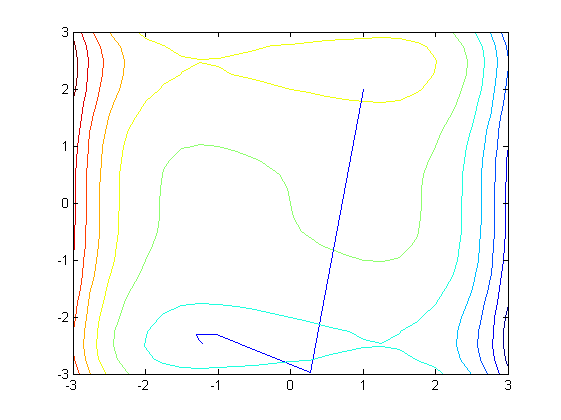
\includegraphics[width=12cm]{fcja2} 
\caption{Wykres kolejnych przybliżeń dla funkcji  $x + 10*x - x^5 + y + 10*y^3 - y^5$.}
\label{fig:funkcja_2}
\end{figure}

Testowana funkcja : $x - x^{3} +y+10*y^{4}$\\
Dla Argumentów : $[-2;-2]$, $x - x^{3}+y+10*y^{4}$, $0.6$ ,$0.99$, $[0.6;0.4]$, $15$, $0.00001$\\
Kolejne przybliżenia:
\begin{enumerate}
\item f(-1.958,-0.792)=164.000
\item f(-0.538,-0.784)=8.694
\item f(-0.538,-0.784)=2.608
\item f(-0.558,-0.635)=2.608
\item f(-0.570,-0.544)=0.608
\item f(-0.577,-0.466)=-0.055
\item f(-0.581,-0.406)=-0.380
\item f(-0.581,-0.362)=-0.519
\item f(-0.580,-0.332)=-0.575
\item f(-0.579,-0.313)=-0.596
\item f(-0.578,-0.302)=-0.602
\item f(-0.578,-0.297)=-0.604
\item f(-0.578,-0.294)=-0.604
\item f(-0.577,-0.293)=-0.604
\item f(-0.577,-0.293)=-0.604
\end{enumerate}

\begin{figure}[H]
\centering
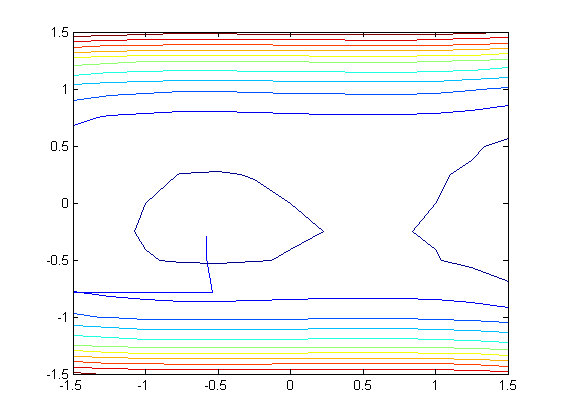
\includegraphics[width=12cm]{fcja3} 
\caption{Wykres kolejnych przybliżeń dla funkcji $x - x^3 +y+10*y^4$.}
\label{fig:funkcja32}
\end{figure}

\begin{table}[H]
	\begin{center}
	\begin{tabular}{|c|c|c|}
	\hline $f(x,y)$ & punkt & wartość w punkcie \\ 
	\hline $x^2+y^2$ & (0,0) & 0 \\ 
	\hline $x + 10*x - x^5 + y + 10*y^3 - y^5$ & (-1.218,-2.456) & -71.958 \\ 
	\hline $x - x^3 +y+10*y^4$ & (-0.577,-0.293) & -0.604 \\ 
	\hline 
	\end{tabular}
	\caption{Zestawienie wyników uzyskanych przy pomocy WolframAlpha }.
	\label{wolfram}
	\end{center}
\end{table}
\section{Wnioski}
W problemie optymalizacji funkcji wielu zmiennych, możemy mieć przypadki trudne do rozstrzygnięcia posiadając jedynie informacje o przegięciu wartości pierwszej pochodnej w punkcie. Przypadkiem takim może być punkt przegięcia który jest punktem ekstremalnym ale nie jest on ani minimum ani maksimum danej funkcji. Wartość przybliżona macierzy Hessego w punkcie rozstrzyga ten problem. Jednakowo wprowadza nową informacje dotyczącą przebiegu badanej funkcji - jej krzywiznę.

Zaprezentowana tutaj metoda wyznacza wartość przybliżoną macierzy Hessego metodą Davidon-Fletcher-Powell \cite{2}, jak widać na prezentowanych rzutach funkcji udało znaleźć się lokalne minima z zadowalającą dokładnością (zgodnie z wynikami wzorcowymi zawartymi w tabeli \ref{wolfram}).

\begin{thebibliography}{9}
\bibitem{1} \url{http://en.wikipedia.org/wiki/Quasi-Newton_method}
\bibitem{2} \url{http://en.wikipedia.org/wiki/DFP_updating_formula}
\bibitem{3} \url{http://en.wikipedia.org/wiki/Wolfe_conditions}
\end{thebibliography}
\end{document}